\chapter{Architecture of the Proxima editor} \label{chap:proxArch}

\bc
Multiple presentations? Will this be hard to implement?

ref to reqs and how the architecture helps?

Partial? is that really when high -> low + extra???
Partial: compare with window that shows only part of the source?

SOMEWHERE: presentation may support duplicates in future, otherwise tree views need enriched 
 document structures.

TODO: mention that font query in arranger is also ui dependent.

TODO: find out where edit gesture/operation should be mentioned

plaatje Proxima + style (parsing) sheet + computation (reduction) sheet -> editor mention Bootstrapping problem, descr. of levels layers and edit model. second is easier to give with in a

formal story. however, design reasons for first are hard to comprehend without idea. So first informal arch 
 and edit model and later the formal stuff
\ec



% Explain tokens more general?
%***** Mention more explicitly that formalisms are AG? elegant efficient. pres more info in Xprez chapter.

A generic editor is a large system consisting of many components. In this chapter, we focus on those components of the Proxima architecture that are involved in the process of presenting the internal document to the user, and interpreting the edit gestures given by the user. Of course, other functionality, such as IO handling, macro processing, or a search facility, is also important for the usability of the final editor, but implementation of these features is largely straightforward, despite the fact that it may require a substantial amount of engineering. The presentation of the document and the handling of edit gestures, on the other hand, is of paramount importance, because it determines for which applications the editor can be used, as well as how powerful the editing behavior will be.

The core architecture of Proxima consists of a number of layers, which only communicate with their direct neighbors. This layered structure is based on the staged nature of the presentation process. Instead of mapping a document directly onto its final rendering, it is first mapped onto an intermediate data structure. This intermediate data structure is mapped onto another intermediate data structure, until the last intermediate data structure is mapped onto the rendering.

As we mentioned in Chapter~\ref{chap:introduction}, the positions at which the document, the rendering, and the intermediate data structures reside are called {\em data levels}. Between each pair of levels is a {\em layer}, which is a component that maintains the mappings between the levels. Figure~\ref{proxlayers} schematically shows the levels and layers of Proxima. Only two data levels are visible to each layer: a higher and a lower level.

\begin{figure}
\begin{center}
%\begin{tabular}{c}
%\framebox[5cm][c]{Document level}\vspace{1ex}\\
%{Evaluation layer}\vspace{1ex}\\
%\framebox[5cm][c]{Enriched document level}\vspace{1ex}\\
%{Presentation layer}\vspace{1ex}\\
%\framebox[5cm][c]{Presentation level}\vspace{1ex}\\
%{Layout layer}\vspace{1ex}\\
%\framebox[5cm][c]{Layout level}\vspace{1ex}\\
%{Arrangement layer}\vspace{1ex}\\
%\framebox[5cm][c]{Arrangement level}\vspace{1ex}\\
%{Rendering layer}\vspace{1ex}\\
%\framebox[5cm][c]{Rendering level}
%\end{tabular}
\begin{center}
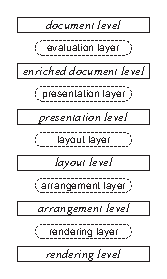
\epsfig{file=pics/eps/LevelLayerNames.eps, width=4cm}
\end{center}
\caption{The levels and layers of Proxima.}\label{proxlayers} 
\end{center}
\end{figure}
% add arrows for pres and interpr.

%sheets?

%\pagebreak \note{watch this pagebreak}
\finallongpage

There are several reasons why the Proxima architecture is layered: 

\begin{description}

\item[Staged presentation process.]
The presentation process is naturally staged. The process consists of repeatedly mapping  structures that have a different meaning on a higher level onto a common set of lower level structures. For example, a table of contents, once its structure has been computed, can be presented in the same way as a chapter structure. Similarly, a line that comes from a formatted paragraph is rendered in the same way as a line that was explicitly specified in the presentation. Mappings like these form stages in the presentation process that can be performed by separate layers.

\item[Specification of presentation and edit behavior.]
A layered architecture provides natural hooks for the editor designer to specify specific parts of the presentation and edit behavior. A separate evaluation layer, makes it possible to separate computation and presentation, thus allowing different style sheets to be used for a document together with its derived structures. At the same time, layers offer more control over backward mappings, such as the specification of how edit operations on derived structures are to be interpreted as edit operations on the document.

\item[Extra state.]
An important aspect of the Proxima editor is the concept of {\em extra state}, which is inherently connected to a layered architecture. If information on a level cannot be computed by presenting the level above, it is presentation extra state, and if it cannot be computed by interpreting the level below, it is interpretation extra state.

\item[Maintaining bidirectional mappings.]
Because Proxima supports editing on all levels, a mapping between each pair of levels needs to be maintained. Maintaining such mappings is easier in a layered architecture. Furthermore, the lower layers can maintain the mappings automatically.

\item[Efficiency.]
Some steps in the presentation process, especially in the higher layers, may be time consuming because global computations need to be performed. In a layered architecture, it is possible to perform the higher layer computations not at every keystroke, but only once in a while. For example, in a program editor, parsing the program may be delayed until the user enters a whitespace character or performs a navigation operation. Type checking the program may be delayed until after a certain period of inactivity, or when requested by the user.
\end{description}

The remainder of this chapter contains an informal description of the levels and layers in the Proxima architecture. A more formal specification of the editor is provided in Chapter~\ref{chap:formalSpec}, preceded by an informal introduction in Chapter~\ref{chap:informalSpec}.


%																
%																
%																
\section{The levels of Proxima}

A data level in Proxima is not just an intermediate value in the presentation computation, but an entity in its own right. Together, the data levels constitute the state of the editor. The six data levels of Proxima are:


\begin{description}
\item[Document:] The edited document, the type of which is specified by a DTD or an EBNF grammar.

\item[Enriched Document:] The document enriched with computed information.

\item[Presentation:] A logical description of the presentation of the document, consisting of rows and columns of presentation elements with attributes. The presentation also supports formatting based on available space (e.g.\ line/page breaking).

\item[Layout:]  Presentation with explicit whitespace.

\item[Arrangement:] Formatted presentation with absolute size and position information.

\item[Rendering:] A collection of user interface commands for drawing the absolutely positioned and sized arrangement.
\end{description}

In the discussion below, we illustrate the different data levels with examples. Note that when an element at one level is mapped onto elements at another level, an implementation will have to keep track of information about this mapping. For simplicity, the details regarding such mapping information have been left out of the examples.

%																
\subsection{Document} \label {sect:docLevel}

A document is the internal tree data structure that is edited by the user. The type of the document is specified by a context-free grammar, with special constructs for lists and optional values (similar to EBNF). Haskell data types, EBNF, DTDs and XML Schemas are all, possibly restricted, forms of context-free grammars suitable for describing the document type. In this thesis, we make use of simple monomorphic Haskell data types together with the list type.

The exact type formalism is important for document to document transformations (i.e.\ document-oriented edit operations), because it should be possible to guarantee type safety of such transformations. However, for the time being, the only supported document-oriented edit operations are simple tree-based operations, such as cut and paste, and basic operations on lists, such as selecting a segment of a list. Therefore, using a context-free grammar formalism for specifying the document structure is expressive enough.
 
Because different instances of a generic editor may have different document types, we give an example document type for a specific instance. The example document consists of a list of declarations, each of which is an identifier declaration or a comment. An identifier declaration contains a string that represents the declared identifier, as well as an expression that consists of conditional expressions, integers, and booleans. The third field of the declaration is a string that contains additional information about the declaration. It is used to illustrate the concept of interpretation extra state in the Proxima editor. A comment consists of a list of strings. The types {\tt String}, {\tt Int}, and {\tt Bool} are primitive types. Although not very suitable for practical purposes, the chosen document type allows us to illustrate the different aspects of the Proxima data levels and layers.

\noindent
\ttfamily
\begin{tabbing}
data Document = Root$_{\Doc}$ [Decl$_{\Doc}$]\\
data Decl$_{\Doc}$ \= = Decl$_{\Doc}$ String Exp$_{\Doc}$ String\\
                            \> | Comment$_{\Doc}$ [String]\\
data Exp$_{\Doc}$ \= =  IfExp $_{\Doc}$ Exp$_{\Doc}$ Exp$_{\Doc}$ Exp$_{\Doc}$\\
                 \> | IntExp$_{\Doc}$ Int\\
                 \> | BoolExp$_{\Doc}$ Bool\\
\end{tabbing}
\rmfamily

The explanation of the presentation process in Section~\ref{sect:presprocess} provides an example document of this type, as well as examples of the lower levels.

%																
\subsection{Enriched document} \label{sect:enrLevel}
\finalshortpage

An enriched document is a copy of the document to which derived information has been added. In the word processor example, the enriched document contains a table of contents, and each section or subsection element has a field that contains its number. Such derived information is not present at the document level.

Besides containing extra information, the enriched document, or a subtree of it, may also be a reordered version of the document. For example, if the document contains a list of elements, the enriched document may contain a sorted list of these elements.

As an example of an enriched document type, we take the document type of the previous section and add a type declaration alternative {\tt TypeDecl} to the {\tt Decl} type. The type declaration is inferred for each declaration. The type of an expression may be integer, boolean, or erroneous (e.g.\ the type of {\tt if True then 0 else False}). It is also possible to add the type as a field to the {\tt Decl} alternative, but separate type declarations make it easier to show how edit operations targeted at the enriched document are handled in Section~\ref{sect:reducer}.

\noindent
\ttfamily
\begin{tabbing}
data EnrichedDocument = Root$_{\Enr}$ [Decl$_{\Enr}$]\\
data Decl$_{\Enr}$ \= = TypeDecl$_{\Enr}$ String Type$_{\Enr}$\\
                           \> | Decl$_{\Enr}$ String Exp$_{\Enr}$ String\\
                           \> | Comment$_{\Enr}$ [String]\\
data Exp$_{\Enr}$ \= =  IfExp $_{\Enr}$ Exp$_{\Enr}$ Exp$_{\Enr}$ Exp$_{\Enr}$\\
                 \> | IntExp$_{\Enr}$ Int\\
                 \> | BoolExp$_{\Enr}$ Bool\\
\\
data Type$_{\Enr}$ = IntType$_{\Enr}$ | BoolType$_{\Enr}$ | ErrorType$_{\Enr}$
\end{tabbing}
\rmfamily


%																
\subsection{Presentation} \label{sect:presLevel}

%what is presentation
A presentation is an abstract description of what the document will look like to the user. It consists of strings, images, and simple graphical elements (lines, boxes, etc.), which are grouped in rows, columns and matrices. A presentation element has attributes for colors, line styles, fonts, and alignment. Attribution may be influenced using a {\em with} element, which contains a rule that specifies how the attribution is affected.

There are three ways of positioning elements in the presentation. Firstly, the position can be specified relative to other elements in the presentation, by placing a list of elements next to each other in a {\em row}, or above each other in a {\em column}. Elements are aligned according to reference lines (e.g.\ the baseline for a string), and stretchable elements may be used to influence the positioning. Besides rows and columns, a {\em matrix} construct presents a list of lists of elements aligned both horizontally as well as vertically, and an {\em overlay} presents a list of elements in front of each other (e.g.\ for presenting a squiggly \makebox(0,0)[lt]{\epsfig{file=Pics/eps/squiggly.bmp.eps, width=0.042in}\epsfig{file=Pics/eps/squiggly.bmp.eps, width=0.042in}\epsfig{file=Pics/eps/squiggly.bmp.eps, width=0.042in}\epsfig{file=Pics/eps/squiggly.bmp.eps, width=0.042in}\epsfig{file=Pics/eps/squiggly.bmp.eps, width=0.042in}}line). 
%mention that alignment is modified easily?

The second way of positioning presentation elements is by using a {\em formatter} element, which positions a list of elements based on the available space. Currently, Proxima only supports horizontal formatting, suitable for line breaking in a paragraph. Vertical formatting (for page breaking) is not fundamentally different, but has not been implemented yet. Furthermore, support for a page model also requires extensions to the lower levels, which have not been realized yet.

Finally, a presentation (or part of it) may consist of a list of tokens, which may be identifiers, operators, integers, strings, etc. Token-list presentations support presentation oriented editing; on interpretation, the (possibly edited) token list is parsed. Each token contains information about the whitespace (line breaks and spaces) that precedes the token in the presentation. This whitespace is an example of presentation extra state, since it is not stored in the enriched document. 

\bc f textual editing on a presentation is desired (e.g.\ for a source editor), a parser is invoked on the presentation after it has been edited. A presentation that needs to be parsed consists of tokens,****** which make it possible to use a separate layer for scanning. \ec

\bc In some cases, a presentation may need to be parsed without using the Proxima scanner. For example, when explicit whitespace information is stored in the document. In that case, dummy tokens that are not processed by the scanner may be used for the presentation. \ec

A presentation consisting of tokens may contain parts that we do not want to be parsed. For example, a textual source editor may have a non-textual presentation for fractions ($\frac{1}{1+x}$). Such a presentation can be included in the token list presentation with a {\em structural token}. A structural token contains a presentation, and is treated specially by the parser. Although a structural presentation itself is not parsed, it may contain other token lists that will be parsed (e.g. the numerator and denominator of the fraction may be parsed again).

Unlike the document and the enriched document, the presentation has a fixed type, of which we present a slightly simplified subset here. The details of the attribution (e.g.\ color, font, and reference lines) of presentation elements have been left out by leaving the type \verb|AttributionRule| abstract. Chapter~\ref{chap:presenting} provides a discussion of these details. 


\noindent
\ttfamily
\begin{tabbing}
data Presentation \= = Empty$_{\Pres}$\\
                  \> | String$_{\Pres}$ String \\
                  \> | Tokens$_{\Pres}$ [Token]\\
                  \> | Row$_{\Pres}$ [Presentation]\\
                  \> | Column$_{\Pres}$ [Presentation]\\
                  \> | Overlay$_{\Pres}$ [Presentation]\\
                  \> | Matrix$_{\Pres}$ [[Presentation]]\\
                  \> | Formatter$_{\Pres}$ [Presentation]\\
                  \> | With$_{\Pres}$ AttributionRule Presentation\\
\\
data Token \= = UCaseToken Whitespace String\\
           \> | LCaseToken Whitespace String\\
           \> | IdentToken Whitespace String\\
           \> | OpToken Whitespace String\\
           \> | IntToken Whitespace Int\\
           \> | StructuralToken Whitespace Presentation\\
           \> \dots \\
\\
type Whitespace = (LineBreaks, Spaces)\\
type LineBreaks = Int\\
type Spaces = Int\\
\\
data AttributionRule = \dots\\
\end{tabbing}
\rmfamily


%																
\subsection{Layout}

The layout level is the same as the presentation level, except that there are no tokens anymore. Each token has been replaced by its string, and its whitespace has been replaced by strings of spaces and by starting a new row for each line break. Thus, at the layout level, all whitespace is explicit. Formatters are still present, because the exact size and position information required to remove them is not known at the layout level.

The similarity between the layout and the presentation level is clearly visible in the types: the {\tt Layout} type is the {\tt Presentation} type without the {\tt Tokens} alternative.

\noindent
\ttfamily
\begin{tabbing}
data Layout \= = Empty$_{\Lay}$\\
            \> | String$_{\Lay}$ String \\
            \> | Row$_{\Lay}$ [Layout]\\
            \> | Column$_{\Lay}$ [Layout]\\
            \> | Overlay$_{\Lay}$ [Layout]\\
            \> | Matrix$_{\Lay}$ [Layout]\\
            \> | Formatter$_{\Lay}$ [Layout]\\
            \> | With$_{\Lay}$ AttributionRule Layout\\
\\
data AttributionRule = \dots\\
\end{tabbing}
\rmfamily


%																
\subsection{Arrangement}

%what is arrangement  : fixed position + size. also formatters are replaced by columns of rows
At the arrangement level, each element gets its position and size. The position is expressed in actual coordinates. These coordinates do not necessarily correspond to pixel coordinates because the rendering may be scaled. 

Because the final positions have been determined, the distinction between rows, columns, etc. is no longer necessary at the arrangement level. Instead, all composite elements are represented by a {\tt Node}, which contains a list of child arrangements.  

Formatters have been resolved and are represented by a single node containing a list of nodes that represent the formatted lines (see Section~\ref{sect:arranger} for an example). The neutral empty element of the layout is not visible and therefore not part of the arrangement type.

% A page model is not yet part of the arrangement.
The arrangement has a tree rather than a list structure to enable the specification of properties, such as font and color information, for an entire subtree, instead of separately for each element of the arrangement. Moreover, a tree structure is helpful for incremental arranging, in which only part of the arrangement is recomputed after an edit operation, whereas the rest is simply copied from the previous arrangement.

% why a tree
Although the coordinates of each element in the arrangement are absolute, the coordinates are represented in the arrangement data structure relative to the coordinates of the parent in the tree. Relative positioning makes it easier to reposition a subtree in the arrangement, because it removes the need to update the position of each element in the moved subtree. 

A \verb|With| node does not have a geometry field, because it only influences the attribution of the arrangement tree, without being an actual part of the arrangement. 
%\nonote{why is geometry of children not part of the node? Answer: because of with nodes}

% debugging?

\ttfamily
\begin{tabbing}
data Arrangement \= =  String$_{\Arr}$ Geometry String\\
                 \> | Node$_{\Arr}$ Geometry [Arrangement]\\
                 \> | With$_{\Arr}$ AttributionRule Arrangement\\
\\
type Geometry = (Position, Size)\\
type Position \= = (Int, Int)  ~~~~~~-- (x,  y)\\
type Size      \> = (Int, Int)  ~~~~~~-- (width, height)\\
\\
data AttributionRule = \dots\\
\end{tabbing}
\rmfamily

%																
\subsection{Rendering}

A rendering is a set of user-interface drawing commands that actually draw on the screen. Positions are expressed in pixel coordinates. In contrast to the other levels, a rendering is a list rather than a tree. However, in the future it may change to a tree structure, to support incremental updates on the rendering. 

Because the rendering is highly dependent on the GUI library that is used, we only give an abstract type.

\noindent
\ttfamily
\begin{tabbing}
type Rendering = [RenderingCommand]\\
data RenderingCommand = \dots
\end{tabbing}
\rmfamily




%																
%																
%																
\section{Editing on different levels in Proxima}

Before we proceed with a description of the layers, we briefly discuss which levels can be edited in Proxima. When a level is targeted by an edit operation, the edit operation is directly performed on that level. Afterwards, the other levels are updated indirectly, as a result of the interpretation and presentation processes. To offer document-oriented as well as presentation-oriented editing, several levels may be targeted in Proxima. However, on some levels it does not make much sense to support direct editing, whereas on others the semantics of direct editing is not clear. We briefly discuss how each level may be edited, starting with the rendering.

\head{Rendering}

A direct edit operation on the rendering would consist of moving around bitmaps, after which the updated rendering needs to be interpreted to yield a new arrangement. The semantics of such edit behavior are unclear and supporting it will probably be difficult, and since direct rendering editing is not required by any of the use cases that drive the design of Proxima (Section~\ref{sect:usecases}), it is not supported.
  
  
\bc
The arrangement level is structurally very similar to the presentation level, except that line breaking has been performed and elements have absolute positions. Edit operations targeted at the arrangement are edit operations concerned with lines and absolute positions, such as navigating to the end of the line that contains the focus, or selecting all elements in a rectangular area.
\ec
%\finallongpage
\head{Arrangement}

Proxima does not support direct editing at the arrangement level. It is not possible to update the arrangement level and compute an edit operation on the presentation level. Edit operations targeted at the arrangement only involve the focus. A consequence is that although rectangular areas may be selected and deleted (the deletion takes place at a higher level), it is not possible to insert a rectangular area. Such edit behavior, often referred to as column editing in text editors, is not a strong requirement for Proxima. In text editors, column editing is used to edit a text that is organized in columns, but since Proxima is a structure editor, a document that has data that needs to be presented in columns can use a presentation-level matrix, the elements of which can be selected column-wise at presentation level.


\head{Layout}

The layout level is the lowest level that can be edited directly. All presentation-oriented editing takes place at the layout level. This includes entering program text in a source editor, but also text entry in the tax form editor or the word processor. Besides text insertion and deletion, also cut, copy and paste operations are supported.

\head{Presentation}

The presentation level does not need to be edited directly because of its direct correspondence to the layout level. Any edit operation that needs to be performed on the presentation level can be performed on the layout level.

\bc The only difference between the two is that the presentation contains lists of tokens that are represented by strings and explicit whitespace in the layout level. Hence the only reason for supporting direct presentation-level editing is for manipulating tokens as lists, which is possible at the layout level as well. \ec

\head{Enriched document and Document}

Because the enriched document and the document are both trees, the edit functionality on both levels is similar. The only difference between the two is that if the enriched document is edited, a subsequent interpretation takes place to compute the document update. Because of the similarities, both levels are discussed together.
% mention isomorphic parts?

The edit operations at the document level are basic tree operations, such as cut, copy and paste on subtrees. If a list element has a parent that is also a list (eg.\ a list of subsections in a list of sections), split and join operations can be applied. An editor designer may specify additional generic or domain-specific transformations.

%\finallongpage
%placeholders
For any element except a list, all child elements are required to be present and hence cannot be left out of the parent element. In order to still be able to manipulate an element without its children, Proxima employs the concept of a placeholder (also found in the Synthesizer Generator~\cite{reps84synGen}). A placeholder of a type $T$ is a dummy value that can be used in any place where an element of type $T$ is required. A document containing a placeholder is incomplete. The placeholders are typically only present during the construction of a document (or part of it), or as an intermediate situation during a document modification that consists of several steps. Lists and optional types do not require placeholders: for a list type, the empty list is the placeholder, and for an optional it is the empty alternative.

\bc %also higher
For example, moving a section entry in a table of contents is a direct edit operation on the enriched document level. An indirect document edit operation that moves the corresponding section (rather than just the entry) is computed from it by the reducer. Because the levels below the targeted level are skipped during interpretation in this case, these levels are not updated until the document is presented again.  \ec

\bigskip

Summarizing, the following three levels may be directly edited in Proxima:

\begin{description}
\item[Layout.] Mainly text-oriented editing, such as entering keywords (e.g.\ "\verb|if|", "\verb|then|", or "\verb|else|") or moving the focus downward one line.
\item[Enriched Document.] Tree edit operations on derived structures, such as moving an entry in a generated table of contents.
\item[Document.] Tree edit operations, such as moving a section in word-processor document; deleting a declaration in Haskell source; or moving the focus to a certain subtree of the document.
\end{description}






%																
%																
%																
\section{The layers of Proxima} \label{sect:archProximaLayers}

Between each pair of data levels is a {\em layer} that takes care of mapping the higher level onto the lower level (downward mapping, or {\em presentation}) and that maps edit operations on the lower level onto edit operations on the higher level (upward mapping, or {\em interpretation}). A layer consists of two components: one for presentation, and one for interpretation. 

In the actual architecture, the downward mapping is not a mapping between the higher and lower levels, but between edit operations on those levels, similar to the upward mapping. Hence, the upward and the downward mappings are symmetrical, as both are concerned with edit operations. 

Besides mapping edit operations onto edit operations, a layer also takes care of updating the data levels by performing the edit operations on them. Data levels are updated on presentation as well as on interpretation. Each layer only updates one of its neighboring levels, because otherwise levels would be updated twice (each level is surrounded by two layers). For implementation reasons that we will not discuss here, a layer component updates its argument level; the presentation component updates its higher level, whereas the interpretation component updates its lower level. 

\bc The exact types of the mappings in a layer are presented in Chapter~\ref{chap:layeredArchs}.\ec 
Figure~\ref{singleLayer} contains a picture of a single layer. In the figure, $level\H$ and $level\L$ denote the higher and lower levels, and $\delta\H$ and $\delta\L$ denote the edit operations on these levels. The $\present$ component computes $\delta\H$ from $\delta\L$, $level\H$ and $level\L$. And, dually, the $\interpret$ component computes $\delta\L$ from $\delta\H$, $level\L$ and $level\H$. The squiggly arrows ($\leadsto$) denote that $\present$ updates $level\H$ and $\interpret$ updates  $level\L$. 
\finalshortpage

\begin{figure}
\begin{small}
\begin{center}
\begin{center}
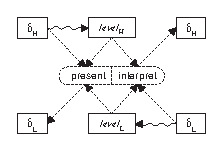
\epsfig{file=pics/eps/ArchLayerSingle.eps, width=5cm} % visio: LayerOverview.vsd
\end{center}\caption{A single Proxima layer}\label{singleLayer} 
\end{center}
\end{small}
\end{figure}
\bc
\begin{figure}
\begin{small}
\begin{center}
\begin{tabular}{ccc}
$\delta_{High}$ & $\leadsto$ \hspace{3.5em} higher level \hspace{5em} & $\delta_{High}$\\
$\downarrow$ & $\swarrow \hspace{3.5em} \searrow$ & $\uparrow$ \\
\multicolumn{3}{c}{ \framebox[8cm][c]{presentation component / ~~interpretation component}\vspace{1ex}}\\
$\downarrow$ & $\nwarrow \hspace{4.0em}  \nearrow$ & $\uparrow$\\
$\delta_{Low}$ &  \hspace{5em}{lower level} \hspace{3.5em}$<\sim$ & $\delta_{Low}$
\end{tabular}
\caption{A single Proxima layer (draft)}\label{singleLayer} 
\end{center}
\end{small}
\end{figure}
\ec
\
\bc
Three kinds of arrows are visible in the picture: downward, upward, and horizontal arrows pointing to the
right. The downward arrows represent the presentation process and the upward arrows represent the
interpretation of edit operations. The horizontal arrows  and the horizontal arrows 

A mapping between edit operations is at least as expressive as a mapping between values, because any 
mapping on values can be represented by a mapping 
%TODO when uncommenting the following, fix math spacing
$f :: Data_{High} \rightarrow Data_{Low}$ can be expressed as a mapping on edit operations
$f' ::  \delta_{Data_{High}} \rightarrow \delta_{Data_{Low}}$ with $f' edit_{High} = set (f (edit_{High}high))$
\ec

%thing is parameterized!!!


\finalshortpage

Because each layer connects two levels and Proxima  consists of six data levels, we have five layers, one for each of the following steps: evaluation, presentation, layout, arrangement and rendering.

Some of the components in the architecture are parameterized with so called {\em sheets}, which describe the specifics of a particular editor instance, similar to style sheets in a web browser. Together with the document type definition, the sheets determine the editor instance. Currently, the evaluation layer has an {\em evaluation sheet} and a {\em reduction sheet} and the presentation layer has a {\em presentation sheet} and a {\em parsing sheet}.  The layout layer, on the other hand only has a {\em scanning sheet}, and the lower layers do not have any sheets at all. 

The presentation sheet is specified by an attribute grammar, whereas the parsing sheet is specified using a Haskell parser combinator library. Section~\ref{sect:instantiating} provides example fragments of presentation and parsing sheets from the Proxima prototype. The formalisms for the evaluation, reduction, and scanning sheets have not been established exactly yet.

The reason why some components do not have sheets is that as of yet no sensible purpose has been found for them. The components without sheets can realize the required mappings without the need for parameters specific to a particular editor instance. However, a future version of Proxima may also support layout sheet and sheets for the lower levels. A layout sheet could be useful for specifying token based syntax coloring, whereas a rendering sheet could be used to specify rendering details, such as the rounding of corners in line drawings.

\begin{figure}
\begin{small}
\begin{center}
\begin{center}
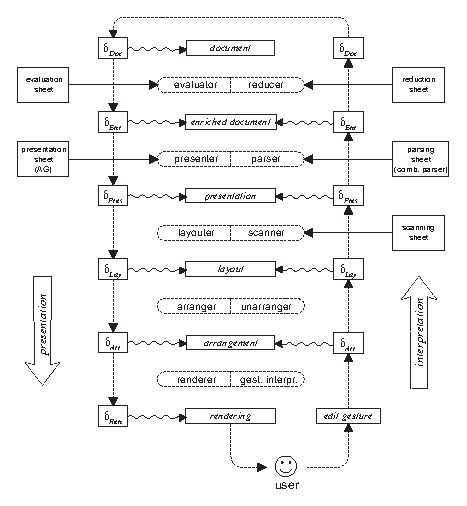
\epsfig{file=pics/eps/ArchLayerOverview.eps, width=8cm} % visio: LayerOverview.vsd
\end{center}\caption{The layers of Proxima.}\label{proxLayers} 
\end{center}
\end{small}
\end{figure}

Figure~\ref{proxLayers} shows an overview of the layers of Proxima. For clarity, the arrows between the layers and the levels are omitted, and a single arrow is used to denote the arrows between the layers and the edit operations. Because the edit gesture is not an edit operation on the rendering, it has no update arrow ($\leadsto$). Furthermore, because the document only needs to be updated once, there is no update arrow on the top-right of the figure. Instead, $\delta_{Doc}$ is passed on to the evaluator, which performs the edit operation on the document.

The downward mappings from all layers together form a logical whole (the presentation process), as do the upward mappings (the interpretation process). Therefore, rather than discussing the components pairwise from layer to layer, we give a description of all the components involved in the presentation process, followed by the components of the interpretation process. 

The examples accompanying the component descriptions show a few instances of both presentation and interpretation extra state. Section~\ref{sect:extraState} discusses extra state in more detail and Section~\ref{sect:singleExtra} provides a formal specification. 

\bc
\begin{description}
\item [Evaluation, Evaluator:] Computes all derived values and structures and may reorder parts of the document. Parameterized with an {\em evaluation sheet}, which specifies the computations.
\item [Evaluation, Reducer:] Maps edit operations on derived structures onto edit operations on the document. Parameterized with a {\em reduction sheet}, which specifies how to handle editing of derived values/structures.
\item [Presentation, Presenter:] Computes the presentation of the enriched document. Parameterized with a {\em presentation sheet}, which is an attribute grammar that , 
\item [Presentation, Parser:] Parsing sheet.
\item [Layout, Layouter:] Adds explicit whitespace to the presentation.
\item [Layout, Scanner:] Removes the whitespace and recognizes tokens. Scanner sheet.
\item [Arrangement layer.]
Arranger: Performs line-breaking and computes absolute sizes and positions.
Unarranger: Translates absolute positions in edit operations to relative positions.
\item [Rendering layer.]
Renderer: Scales the arrangement and maps it onto user interface drawing commands.
Gesture interpreter: Maps edit gestures onto edit operations targeted at the appropriate levels, and descales positions in edit operations.
\end{description}
\ec


\bc
In the discussion of each of the layers, we present three examples of extra state. For presentation extra state, the example is the (editable) whitespace in the presentation. , whereas the example of interpretation extra state is a partial presentation of the document. Although extra state may also appear at the evaluation layer, both of the examples are in the presentation layer. 
\ec


%																
%																
%																
\section{Presentation process} \label{sect:presprocess}

The presentation process is the stepwise mapping of a document onto its final rendering. Although the mapping is actually a mapping between edit operations on each of the levels, we will present it here as a mapping between levels. The reason for this is that the mapping between edit operations is important mainly for incrementality, and viewing the presentation process as a mapping between levels makes it easier to explain.

In order to illustrate the different stages in the presentation process, we follow the presentation of a simple document. After the description of each layer component, the intermediate result of the presentation of the document is given. 

The document type is the expression list document type from Section~\ref{sect:docLevel}. The document itself consists of two items: a comment and an expression. For brevity, we denote strings on each level with {\tt "\dots"} instead of {\tt String$_{\Level}$ "\dots"}. Note that the comment is part of the document, unlike comments in regular programs.

Document:
\small \ttfamily
\begin{tabbing}
Root$_{\Doc}$ \= [ Comment$_{\Doc}$ ["This", "is", "a", "simple", "expression"] \\
       \> , Decl$_{\Doc}$ \= "simple1" \\
       \>                        \>(IfExp$_{\Doc}$ (BoolExp$_{\Doc}$ True) (IntExp$_{\Doc}$ 1) (IntExp$_{\Doc}$ 0))\\
       \>                        \> "info"\\
       \> ] 
\end{tabbing}
\rmfamily \normalsize

To a user, this document appears as:\\

\begin{center}\framebox{
\begin{minipage}[t]{1.15in}
This is a simple
\hbox{expression}\\
\\
\ttfamily
\hbox{simple1~::~Int}\\
\hbox{simple1~=} \\
\hbox{~~if~True~then~1}\\
\hbox{~~~~~~~~~~else~0}
\end{minipage}
}
\end{center}

%																
\subsection{Evaluation layer: Evaluator} \label{sect:evaluator}

%what is evaluator
The first step in the presentation process is the computation of the derived information in the document. The component that takes care of this is the evaluator. The evaluator is parameterized with an {\em evaluation sheet}, which is a declarative specification of the derived values. The evaluation sheet may be specified with an attribute grammar, but no final choice for the formalism has been made yet.

Besides basic values, such as section numbers or the outcome of a computation in a spreadsheet, the evaluator may also derive tree structures, such as a table of contents. The derived structures may be partial, duplicated, or reordered versions of the document.

%.computing values, type errors , page numbers, table of contents
\bigskip {\bf Example:} For each declaration, the evaluator computes a type declaration in the enriched document. In the example this means that a type declaration for \verb|"simple1"| with type {\tt IntType} is included in the item list.

Enriched document:
\small \ttfamily
\begin{tabbing}
Root$_{\Enr}$ \= [ Comment$_{\Enr}$ [ "This", "is", "a", "simple", "expression" ]\\
       \> , TypeDecl$_{\Enr}$ "simple1" IntType$_{\Enr}$\\
       \> , Decl$_{\Enr}$ \= "simple1"\\
       \>                       \> (IfExp$_{\Enr}$ (BoolExp$_{\Enr}$ True) (IntExp$_{\Enr}$ 1) (IntExp$_{\Enr}$ 0)) \\
       \>                        \> "info"\\
       \> ] 
\end{tabbing}
\rmfamily \normalsize


%																
\subsection{Presentation layer: Presenter} \label{sect:presenter}

%what is presenter
The enriched document is mapped onto the presentation by the presenter. Similar to the evaluator, the presenter is parameterized with a {\em presentation sheet} that specifies the presentation. The presentation sheet is an attribute grammar that defines the presentation as a synthesized attribute for each element in the enriched document. 

In order to support extra state, the presentation layer keeps track of the mappings between the elements of the enriched document and the elements of the presentation. The presenter stores the enriched document origin in each presentation element, whereas the parser stores the presentation elements that were used for parsing in the enriched document.

Tokens are an example of presentation extra state in the presenter, because a token contains its own whitespace, which is not represented in the document or enriched document levels. If an enriched document structure is re-presented, the original tokens (and corresponding white\-space) are reused. 

%\finallongpage
If an enriched document element that is presented with tokens, is newly created or has not been presented before, a default value for the whitespace of its tokens is chosen. This default may come from a pretty printing algorithm. A default value may also be used in case a structure has been edited in such a way that reusing the old tokens does not make sense.

The mechanism of reusing presentation tokens is also used to handle ambiguities in token representations. For example, when a user has entered the text ``001'' which is stored in the document as the integer 1, the mapping between the enriched document and the presentation ensures that on re-presentation, the integer is presented as ``001'' instead of ``1''.

% strongly related to evaluator
The separation between evaluating and presenting is more pragmatic than theoretical. On the one hand, the entire presentation can be regarded as a derived structure, and on the other hand the presentation sheet can reorder elements in the presentation and introduce structures, which is more appropriately done in the evaluation sheet. 

The editor designer must make a careful decision on where to specify document evaluation and presentation. Whenever editing on a derived structure is supported, the computation of the structure must be part of the evaluation. But even if a derived structure is not intended to be editable, it may be wise to compute it during evaluation. Take for example a table of contents or a bibliography in a word processor. If the computation of such a structure is part of the evaluation, then its presentation can be changed without having to know the details of the computation.

\bigskip {\bf Example:} The example presentation of the enriched document is basic: a comment is put in a formatted paragraph and a (type) declaration is presented in a textual infix representation using tokens. The third string field of the declaration \verb|"info"| is not included in the presentation in order to have an example of interpretation extra state. \bc The reason for this becomes apparent in Section~\ref{sect:parser} on parsing.\ec  The pair of numbers in each token represents the whitespace ({\em line breaks}, {\em spaces}) preceding it. This is a rather basic representation, in which spaces at the end of a line cannot be encoded, but for demonstration purposes it is sufficient.

The \verb|With| nodes specify the font for the presentation of the declarations. To keep things simple, the exact details of the attribution rule are not shown: the bracketed declaration \verb|{fontFamily = "|{\em name}\verb|", fontSize = |{\em size}\verb|}| specifies the font family and size for the child of the with node.

Presentation:
\small \ttfamily
\begin{tabbing}
Col$_{\Pres}$ \= [ With$_{\Pres}$ \{ fontFamily = "Times New Roman", fontSize = 12 \}\\
       \>  ~~~ (Formatter$_{\Pres}$ [ "This", "is", "a", "simple", "expression" ])\\
       \>, With$_{\Pres}$ \{ fontFamily = "Courier New", fontSize = 12 \}\\
       \>  ~~~ \= (Tokens$_{\Pres}$ \= [ LCaseToken$_{\Pres}$ (1,0) "simple1",  OpToken$_{\Pres}$ (0,1) "::"\\  
       \>          \>              \> , UCaseToken$_{\Pres}$ (0,1) "Int"\\
       \>          \>              \> ])\\
       \>, With$_{\Pres}$ \{ fontFamily = "Courier New",  fontSize = 12 \}\\
       \>  ~~~ \= (Tokens$_{\Pres}$ \= [ LCaseToken$_{\Pres}$ (1,0) "simple1", OpToken$_{\Pres}$ (0,1) "="\\
       \>          \>              \> , LCaseToken$_{\Pres}$ (1,2) "if", UCaseToken$_{\Pres}$ (0,1) "True"\\
       \>          \>              \> , LCaseToken$_{\Pres}$ (0,1) "then", IntToken$_{\Pres}$ (0,1) "1"\\
       \>          \>              \> , LCaseToken$_{\Pres}$ (1,10) "else", IntToken$_{\Pres}$ (0,1) "0"\\
       \>          \>              \> ])\\
             \> ]
\end{tabbing}
\rmfamily \normalsize


%																
\subsection{Layout layer: Layouter} \label{sect:layouter}

%what is layouter
The layouter processes the tokens in the presentation level, yielding the layout level. Each list of tokens is mapped onto a column that contains rows of strings. The spaces in the whitespace of a token are represented as strings of spaces, whereas line breaks cause new rows in the layout. 

%\finallongpage
Structural tokens are treated specially, because these are not strings. A structural token is represented in the layout level by its {\tt Presentation} field, whereas its whitespace is handled similarly to the other tokens. The presentation of a structural token in the layout level is tagged in order to be able to retrieve the structural token during scanning.

%The layout layer may be parameterized with a layout sheet, in whi


\bigskip {\bf Example:} The tokens in the presentation level are replaced by strings in the layout level (the \textvisiblespace~character denotes a space). The formatter is not affected. The line break before the type declaration is represented by an empty string. 

Layout:
\small \ttfamily
\begin{tabbing}
Col$_{\Lay}$ \= [  With$_{\Lay}$ \{ fontFamily = "Times New Roman", fontSize = 12 \}\\
                    \>  ~~~ (Formatter$_{\Lay}$ [ "This", "is", "a", "simple", "expression" ])\\
                    \> , With$_{\Lay}$ \{ fontFamily = "Courier New",  fontSize = 12 \}\\
                    \>  ~~~ \= (Col$_{\Lay}$ \= [ "" \\
                    \>          \>        \> , Row$_{\Lay}$ [ "simple1", "\textvisiblespace", "::",
                                                                           "\textvisiblespace", "Int" ]\\
                    \>          \>        \> ])\\
                    \> , With$_{\Lay}$ \{ fontFamily = "Courier New",  fontSize = 12 \}\\
                    \>  ~~~ \= (Col$_{\Lay}$ \= [ Row$_{\Lay}$ [ "simple1", "\textvisiblespace", "=" ]\\
                    \>          \>        \> , Row$_{\Lay}$  [ "\textvisiblespace\textvisiblespace", 
                                                                             "if", "\textvisiblespace", "True", "\textvisiblespace", 
                                                                             "then", "\textvisiblespace", "1" ]\\
                    \>          \>        \> , Row$_{\Lay}$ [ "\textvisiblespace\textvisiblespace\textvisiblespace
                                                                             \textvisiblespace\textvisiblespace\textvisiblespace
                                                                             \textvisiblespace\textvisiblespace\textvisiblespace                                                                                         \textvisiblespace ", "else", "\textvisiblespace", "0" ]\\
                    \>          \>        \> ])\\
                    \> ]
\end{tabbing}
\rmfamily \normalsize


%																
\subsection{Arrangement layer: Arranger} \label{sect:arranger}

The arranger computes the exact sizes and positions for all elements in the layout level, yielding the arrangement. Fonts are queried to determine the size of strings, and child elements of composite elements such as rows and columns are aligned and positioned.

The arrangement layer also resolves formatters. Based on the amount of available space for a formatter, its child elements are distributed along rows using a (possibly optimal) line-breaking algorithm. These rows are put in a column, and the resulting column of rows is then mapped onto arrangement nodes in the same way as regular rows and columns.


\bigskip {\bf Example:} The formatter, which is the first element in the top-level column of the example layout, is replaced by a node that contains a list of nodes in the arrangement. Furthermore, each element in the arrangement tree has an exact size and a position relative to its parent, which are denoted with superscripts: {\em element}$^{(x,\,y)(\mathit{width}\times \mathit{height})}$. 

Note that the \verb|With| elements are not removed because the font information is required to render the arrangement.

Arrangement:
\small \ttfamily
\begin{tabbing}
Node$_{\Arr}^{(0,0)(80\times84)}$ \\
~ \= [ With$_{\Arr}$ \{ fontFamily = "Times New Roman", fontSize = 12 \}\\
      \> ~~~ (Node$_{\Arr}^{(0,0)(80\times24)}$ \\
      \> ~~~~~~ \= [ Node$_{\Arr}^{(0,0)(80\times12)}$ \= [ "This"$^{(0,0)(17\times12)}$, "is"$^{(25,0)(6\times12)}$, "a"$^{(41,0)(4\times12)}$ \\
      \>       \>                                                      \>, "simple"$^{(53,0)(27\times12)}$]\\
      \>       \> , Node$_{\Arr}^{(0,12)(80\times12)}$  [ "expression"$^{(0,0)(42\times12)}$]\\
      \>       \> ])\\
                    
      \> , With$_{\Arr}$ \{ fontFamily = "Courier New",  fontSize = 12 \}\\
      \> ~~~ (Node$_{\Arr}^{(0,24)(75\times24)}$\\
      \> ~~~~~~ \= [ ""$^{(0,0)(0\times12)}$\\
      \>      \> , Node$_{\Arr}^{(0,12)(75\times12)}$ \= [ "simple1"$^{(0,0)(35\times12)}$, "\textvisiblespace"$^{(35,0)(5\times12)}$, "::"$^{(40,0)(10\times12)}$\\
      \>      \>                                                      \> , "\textvisiblespace"$^{(50,0)(5\times12)}$, "Int"$^{(55,0)(15\times12)}$ ]\\

      \>      \>  ])\\
                    
      \> , With$_{\Arr}$ \{ fontFamily = "Courier New",  fontSize = 12 \}\\
      \> ~~~ (Node$_{\Arr}^{(0,48)(80\times36)}$\\
      \> ~~~~~~ \= [  Node$_{\Arr}^{(0,24)(50\times12)}$ [ "simple1"$^{(0,0)(35\times12)}$, "\textvisiblespace"$^{(35,0)(5\times12)}$, "="$^{(40,0)(5\times12)}$ ]\\
      \>      \> , Node$_{\Arr}^{(0,36)(80\times12)}$ [ \dots~]\\
      \>      \> , Node$_{\Arr}^{(0,48)(80\times12)}$ [ \dots~]\\
      \>      \> ])\\
      \> ]

\end{tabbing}
\rmfamily \normalsize


%																
\subsection{Rendering layer: Renderer} \label{sect:renderer}

The renderer maps each element of the arrangement onto a set of drawing commands for the user interface. While traversing the arrangement, information from the \verb|With| nodes is used to generate commands that set the font, style, and color of the rendering. All positions and sizes have already been computed by the arranger, and the renderer only scales these positions and sizes according to the current scaling factor of the view. 

%rendering sheet: how to render things, e.g.\ corners of lines smooth or not. Maybe not very realistic.

\bigskip {\bf Example:} The result of applying the renderer to the example arrangement is a set of rendering commands that display the comment and the declaration when executed.


Rendering:
\small \ttfamily

[ setFont "Times New Roman" 12,  drawText (0,0) "This", drawText (25,0) "is"\\
, \dots ~]
 
\rmfamily \normalsize
The result of executing these commands was already shown at the start of this section, but for completeness we repeat it here. Note that the comment is rendered in a different font than the declaration. 

\begin{center}\framebox{
\begin{minipage}[t]{1.15in}
This is a simple
\hbox{expression}\\
\\
\ttfamily
\hbox{simple1~::~Int}\\
\hbox{simple1~=} \\
\hbox{~~if~True~then~1}\\
\hbox{~~~~~~~~~~else~0}
\end{minipage}
}
\end{center}

%																
%																
%																
\section{Interpretation process} \label{sect:intrProcess}

The interpretation of edit operations is layered in the same way as the presentation process. However, there are important differences between the two. For the interpretation process, edit operations are the main focus. Therefore we will not view interpretation mappings as mappings between levels (as we did for the presentation process) but as mappings between edit operations. \bc Another difference is that in the interpretation process layers may be skipped. For example, a document-oriented edit operation is passed upwards by the lower layers, until it reaches the evaluation layer, where it is performed on the document level. \ec



An edit operation may be interpreted either {\em indirectly}, or {\em directly} (not to be confused with directly/indirectly editing a level). If an edit operation is interpreted {\em indirectly}, the operation is performed on the lower level, yielding an updated lower level. The updated lower level is then mapped onto a new higher level, from which a higher-level edit operation is computed by taking the difference between the new and the previous higher level.

For an example of indirect interpretation, consider the insertion of a token in the presentation level. 
Rather than mapping this edit operation directly onto an edit operation on the enriched document, the token is inserted in the presentation, the presentation is parsed, and the edit operation is distilled from the new enriched document and its previous value.

An edit operation that is {\em directly} interpreted, on the other hand, is immediately mapped onto an edit operation on the higher level, without first performing the operation on the lower level. An example is the interpretation of a mouse click on a position in the arrangement, which is mapped onto a mouse click on a tree path in the layout level. 

Note the difference between direct or indirect interpretation versus direct or indirect editing. A level is edited directly if an edit gesture is targeted at that level, whereas the level is edited indirectly if it changes due to to an edit gesture targeted at another level. When a certain level is directly edited, this results in direct interpretation by all layers below that level, and indirect interpretation by the layers above. Hence, because the rendering and arrangement levels may not be edited directly, the lowest two layers (rendering and arrangement) only support direct interpretation.

\bc When a level is edited directly, a user may target an edit operation at that level. On the other hand, a level is edited indirectly when it is modified as a result of the interpretation and presentation of  an edit operation targeted at a different level. Hence, when a level is directly targeted by an edit operation, this leads to an indirect interpretation of the edit operation, whereas indirectly editing a level (by targeting another level) may lead to either direct or indirect interpretation. \ec



\bc The reason for this is that the rendering and the arrangement level cannot be edited by the user, and an indirect interpretation only takes place when a lower level is edited and the edited level is then mapped onto the new higher level. The lowest level that may be edited by the user is the layout level. However, the architecture does not fundamentally prohibit editing the lower levels, and a future version of Proxima may support editing on the arrangement, by allowing a user to change the absolute positions of arrangement elements. Editing the rendering seems to be rather far fetched, since this means that a user would modify the image of the rendering (e.g.\ by turning pixels on and off).
\ec



Because the interpretation of edit operations does not always go through all stages like the presentation does, and because of the variation in edit operations, it is not helpful to give a running example of the interpretation process. Instead, a number of separate examples are provided together with the descriptions of the interpretation components.

%																
\subsection{Rendering layer: Gesture interpreter} \label{sect:gestureInterpreter}

The gesture interpreter has two tasks. It maps edit gestures onto edit operations for the designated levels, and it interprets direct edit operations on the rendering as edit operations on the arrangement, which means that absolute positions in pixel coordinates are descaled to arrangement level coordinates. 

\bigskip {\bf Example:} 
We give two interpretation examples for the gesture interpreter: a mouse click and a key press. 

The mouse edit operation is a single left-click at pixel coordinates (84,57) in a rendering that has been scaled to 150\%.
Because of the scaling factor, the coordinates are divided by 1.5 to get the arrangement coordinates.

\ttfamily
MouseClick$_{\Ren}$ Left (84,57) $\mapsto$ MouseClick$_{\Arr}$ Left (56, 38)\\
\rmfamily

The second example is a key press of the letter `\verb|a|', which is mapped onto an insert event. However, a textual insert event is targeted at the layout level instead of the arrangement level, since the arrangement level cannot be edited textually. Because the insert operation is not of the arrangement edit type, it is wrapped with a \p{Wrap$_{\Arr}$} constructor. The arrangement layer will remove the \p{Wrap$_{\Arr}$} constructor and pass the insert operation on to the layout layer.

\ttfamily
KeyPress$_{\Ren}$ 'a' $\mapsto$ Wrap$_{\Arr}$ (Insert$_{\Lay}$ 'a')
\rmfamily


%																
\subsection{Arrangement layer: Unarranger}

The main task of the unarranger is to map locations in arrangement-level edit operations onto locations in layout-level edit operations. A location that is specified in absolute coordinates is first converted to a location in the arrangement tree, which is specified as a tree path. Subsequently, the arrangement tree path is mapped onto a layout tree path. The arrangement tree is largely isomorphic to the layout tree, except for the formatter subtrees, as these are represented by nodes that contain lists of nodes (representing the formatted lines) in the arrangement. Therefore, the mapping is almost the identity function, except for paths to children of nodes originating from a formatter, which are mapped onto paths to the corresponding child elements of the formatter.

\bigskip {\bf Example:}
A left-click mouse event at position (56,38) in the example arrangement from Section~\ref{sect:arranger} represents a click on the string ``\verb|Int|'' in the layout from Section~\ref{sect:layouter}. To be precise, it is a click on the left side of the letter `\verb|I|'. If we represent a path in the arrangement tree by a list of integers and a 0 denotes the first child, then this position is represented by \verb|[1,0,1,4,0]|. Thus:

\small \ttfamily
unarrange (MouseClick$_{\Arr}$ (56,38) Left) = MouseClick$_{\Lay}$ [1,0,1,4,0] Left
\rmfamily \normalsize


%																
\subsection{Layout layer: Scanner} \label{sect:scanner}

%scanner does lexical analysis. 

The scanner is the first layer that supports indirect interpretation, since the layout level may be edited by the user. Edit operations targeted at the layout level are performed on the layout level, after which the level is scanned, yielding the new presentation. An edit operation on the presentation is obtained by taking the difference between the new presentation and its previous value. 

The scanner operates only on the subtrees in the layout layer that originate from a token list on the presentation level, while leaving other parts of the tree unaffected. Every such subtree, which is always a column of rows, is scanned by inspecting it row by row, and recognizing the tokens that are represented by the strings in each row. For each token, the whitespace (spaces and row transitions) preceding it is recorded and stored in the token. The parts of the layout tree that originate from structural tokens, have been tagged by the layouter and are scanned as structural tokens.

If the scanner encounters an error during the scanning process, (e.g.\ in case of an unterminated string), it generates an error token, which will subsequently cause a parse error in the parsing layer. The details of this process are not discussed here. 

The scanner is parameterized with a {\em scanner sheet}, which contains a set of regular expressions describing the allowed set of tokens. Since different parts of a layout may require different scanners (e.g.\ in a presentation that shows both Java and Haskell code), a scanner sheet can contain several sets of token descriptions. The layout level contains information on what kind of presentation gave rise to the parts that need to be scanned, which allows the scanner to use the appropriate set of token descriptions.

Scanning is usually a localized process, so rather than re-scanning an entire token list, only the edited part of the layout level is scanned and used to compute the appropriate presentation-oriented edit commands. An exception to this local behavior is formed by tokens with an explicit start and end tag, such as strings or characters. If a string or character quote is entered, this may affect more than just the edited part of the layout.

The scanner layer does not yet support the handling of comments that may appear anywhere in the source. Because such comments are not part of the document, they need to be handled as presentation extra state, similar to whitespace. Comments may affect the locality of the scanning process in the same way as strings.
\finalshortpage

\bigskip {\bf Example:}
Consider the example layout level from Section~\ref{sect:layouter} and assume that the edit operation on the layout is the insertion of a space between the characters `\p{e}' and `\p{1}' in the identifier ``\verb|simple1|'' of the declaration. Because ``\verb|simple 1 = if |\dots'' is not a valid declaration, the edit operation will cause a parse error in the presentation layer, but this has no consequences for the example at the layout layer.

In order to compute the edit operation on the presentation, we first apply the layout edit operation to the layout level, yielding:

\small \ttfamily
\begin{tabbing}
%Col$_{\Lay}$ \= [ "" \\
                  %\> , Row$_{\Lay}$ [ "simple 1", "\textvisiblespace", "::", "\textvisiblespace", "Int" ]\\
%                  \> ]\\
\dots\\
Col$_{\Lay}$ \= [ Row$_{\Lay}$ [ "simple\textvisiblespace1", "\textvisiblespace", "=" ]\\
                   \> , Row$_{\Lay}$ [ "\textvisiblespace\textvisiblespace", 
                                                 "if", "\textvisiblespace", "True", "\textvisiblespace", \dots ] \\
                   \> \dots ]\\
\dots
\end{tabbing}
\rmfamily \normalsize

%\finallongpage
Now, the scanner is invoked on the updated parts of the layout, which gives rise to the following list of tokens.

\small \ttfamily
\begin{tabbing}
Tokens$_{\Pres}$ \= [ \dots \\
                           \> , LCaseToken$_{\Pres}$ (1,0) "simple", IntToken (1,0) 1,\\
                           \> , OpToken$_{\Pres}$ (0,1) "="\\
                           \> , LCaseToken$_{\Pres}$ (1,2) "if", UCaseToken$_{\Pres}$ (0,1) "True"\\
                           \> \dots ]                      
\end{tabbing}
\rmfamily \normalsize
 
From the new token list and the old presentation, an edit operation on the presentation level can be derived:

\small \ttfamily
\begin{tabbing}
\rmfamily {\em insert$_{\Lay}$} \ttfamily ' ' \\
$\mapsto$\\
\rmfamily {\em replace$_{\Pres}$} \ttfamily [ LCaseToken$_{\Pres}$ (1,0) "simple1" ]\\  
\rmfamily {\em by} \ttfamily [ LCaseToken$_{\Pres}$ (1,0) "simple", IntToken (1,0) 1 ] 
\end{tabbing}
\rmfamily \normalsize

We use an informal notation for both the {\em insert} and the {\em replace} edit operations to improve readability. The actual insert operation also contains a reference to the target location of the inserted character, and the replace operation contains the location of the target token list, rather than the list itself. 


%																
\subsection{Presentation layer: Parser} \label{sect:parser}
        
% mention error correction and other repairing parsers? or do this in conclusions?

It is not possible to map edit operations on the presentation directly onto edit operations on the enriched document. Consider, for example, the insertion of the string ``\verb|if|'' in a source editor. From this insertion command only, we cannot compute an enriched document update. Instead, we need to take the indirect approach: the edit operation is applied to the presentation, which is then parsed to yield a new enriched document. Similar to the scanner, the parser layer computes an edit operation on the enriched document by taking the difference between the new enriched document and its previous value. 

The parser component is parameterized with a {\em parsing sheet}, which contains the actual specification of the parser. The parser is specified in Haskell, using a specialized parser combinator library. The parser combinators from this library parse a presentation tree instead of a string. Furthermore, special support is available for handling interpretation extra state.

The parser makes a distinction between token lists and the rest of the presentation. Only the token lists are actually parsed. The other parts of the presentation may not be edited at the presentation level and are therefore mapped onto their originating enriched document structures. Because parsed presentations may contain parts that are not parsed, and vice versa, the two processes alternate.

Each part of the presentation that is not parsed is mapped directly onto the enriched document element of which it is the presentation. In order to do so, the parser layer uses the information on the enriched document origin that is stored in each presentation element by the presenter.
%\nonote{call this recognizing}

%\finallongpage
If the originating enriched document element has children that are also presented, these children are determined via the same process. A child that does not appear in the presentation is reused from the previous enriched document level, or, if this is not possible, it is initialized to a default value. If a child has a token list presentation, the parser process takes over.

The parser that is applied to the list of tokens is specified  in the parsing sheet. Parse errors are represented in the document by error nodes that may appear anywhere in the document tree. If a \p{StructuralToken} is encountered, the previously described mapping process is invoked again. Because the enriched document may contain information that is not presented (i.e.\ interpretation extra state), the parser tries to reuse the enriched document nodes from the previous version of the enriched document. If a node cannot be reused, the extra information is initialized to a default value. 

In order to support presentation extra state for tokens (e.g.\ whitespace), the parser stores a reference to the parsed tokens in the resulting enriched document node. This information is used when the enriched document is presented. Because currently the only form of presentation extra state is whitespace in tokens, the mapping information only needs to be kept for enriched document elements that are parsed.

\bc
Even though it is possible to specify a presentation for which it is impossible to automatically determine the originating enriched document elements, this need not be a problem. In that case, automatic handling of presentation-oriented editing is not supported, and the editor designer will have to take care of handling it, or prohibit it altogether. \ec

\bigskip {\bf Example:}
We consider a delete operation on a number of successive tokens in the presentation. For simplicity, each declaration or type declaration in our example is presented as a separate token list and will therefore be parsed separately. Thus, presentation-oriented edit operations have to be local to a single declaration. In an actual source editor, the token lists are concatenated, and editing may span several declarations.

The presentation level for the example is the same as in Section~\ref{sect:presenter}. The part that is affected by the edit operation is: 

\small \ttfamily
\begin{tabbing}
\dots\\
Tokens$_{\Pres}$ \= [ LCaseToken$_{\Pres}$ (1,0) "simple1", OpToken$_{\Pres}$ (0,1) "="\\
                         \> , LCaseToken$_{\Pres}$ (1,2) "if", UCaseToken$_{\Pres}$ (0,1) "True"\\
                         \> , LCaseToken$_{\Pres}$ (0,1) "then", IntToken$_{\Pres}$ (0,1) "1"\\
                         \> , LowercaseToken$_{\Pres}$ (1,10) "else", IntToken$_{\Pres}$ (0,1) "0"\\
                         \> ]\\
\dots                                                  
\end{tabbing}
\rmfamily \normalsize

The delete operation removes the \verb|"if"|,  \verb|"True"|,  \verb|"then"|,  \verb|"1"|, and  \verb|"else"| tokens, giving rise to a new presentation level.

\small \ttfamily
\begin{tabbing}
\dots\\
Tokens$_{\Pres}$ \= [ LCaseToken$_{\Pres}$ (1,0) "simple1", OpToken$_{\Pres}$ (0,1) "="\\
                         \> ,  IntToken$_{\Pres}$ (0,1) "0"\\
                         \> ]\\
\dots                                                  
\end{tabbing}
\rmfamily \normalsize

A parser is invoked on the new list of tokens. The result is not an entire enriched document, but only an updated declaration for \verb|simple1|. Interpretation extra state children, such as the third child of the declaration (see the example in Section~\ref{sect:presenter}), are not in the presentation and are therefore reused from the previous value of the declaration. The previous value of the declaration is obtained from a reference that was stored in its tokens on presentation. 
%The string is part of the interpretation extra state at the enriched document level.

\small \ttfamily
\begin{tabbing}
Decl$_{\Enr}$ \= "simple1" (IntExp$_{\Enr}$ 0) "info"
\end{tabbing}
\rmfamily \normalsize

The edit operation is computed from the new enriched document part and the previous enriched document, yielding:

\small \ttfamily
\begin{tabbing}
\rmfamily {\em delete}$_{\Pres}$\ttfamily  "if" \dots~"else"\\
$\mapsto$\\
 \rmfamily {\em replace$_{\Enr}$} \ttfamily (IfExp$_{\Enr}$ (BoolExp$_{\Enr}$ True) (IntExp$_{\Enr}$ 1) (IntExp$_{\Enr}$ 0))\\
 \rmfamily {\em by} \ttfamily (IntExp$_{\Enr}$ 0) 
\end{tabbing}
\rmfamily \normalsize

It should be noted that the second \ttfamily (IntExp$_{\Enr}$ 0)\rmfamily in the replacement operation is exactly the same as the one in the else part of the if expression. In this case, the expression is uniquely determined by its presentation, and hence parsing it gives an exact copy, but even if this were not the case, both expressions would be the same, due to the reuse strategy of the parser. For example, if the integer expression has an extra field that is not presented, the replacement integer expression gets the value for that field from the integer expression in the else part. This is analogous to the \verb|"info"| string for the declaration.

% seems double. The incrementality also offers a kind of reuse.

\bc
After it is edited, an enriched document may be inconsistent with regard to the document. For example, if the declaration is edited in such a way that its type no longer matches the one in its type declaration. The consistency is guaranteed again when the edit operation is interpreted by the reducer and the 
\ec

%																
\subsection{Evaluation layer: Reducer} \label{sect:reducer}

The reducer takes care of mapping edit operations on derived structures onto edit operations on the document. The specification of the mapping is in the {\em reduction sheet}, which in many cases can be automatically derived from the evaluation sheet. Automatic reduction behavior is typically possible for parts of the enriched document that are duplicated, reordered, or partial versions of parts of the document. 

If a document structure is duplicated in the enriched document, and one of the duplicates has been edited, the reducer resolves the situation by taking the duplicate that was edited. If both duplicates have been edited, either the edit operation is blocked, or a choice between the two is made. Reordered and partially presented document structures are handled by maintaining a mapping between each enriched document element and the document element from which it originated.

Although it is possible for a derived structure to be editable, this behavior is not enforced. For many derived structures, a reverse mapping does not make much sense. For example, it is hard to give a clear semantics to the direct editing of a chapter number. However, when two chapters in a table of contents are swapped, swapping the two corresponding chapters in the document could well be the desired effect. When the reverse mapping makes sense, it can be specified in the reduction sheet. When not, editing derived structures can be forbidden.

Besides regarding the reduction as the reverse of the evaluation, it is also possible to use reduction as an extension of the parser. As an example, consider a program source that contains definitions of infix operators with user-specified associativity and precedence. Parsing such operators in one pass requires a sophisticated parser, whereas the two-pass solution is straightforward.

Another application of reduction is the handling of redundancy in a document presentation. For example, when a document type for expressions does not have an explicit representation for parentheses, redundant parentheses that are entered by a user can be removed by the reducer, to be added again by the evaluator.

\bigskip {\bf Example:} 
The example editor supports editing on the function name in a type declaration, which causes an update on the name in the corresponding declaration. 
%Although this may not always be desirable behavior in an actual source editor, it provides a good example of editing on derived values.
The example edit operation is an update on the function name in the type declaration of the enriched document from Section~\ref{sect:evaluator}. The name is changed from \verb|"simple1"| to \verb|"simple"|. Thus, we get the following updated enriched document.

\small \ttfamily
\begin{tabbing}
Root$_{\Enr}$ \= [ Comment$_{\Enr}$ [ "This", "is", "a", "simple", "expression" ]\\
       \> , TypeDecl$_{\Enr}$ "simple" IntType$_{\Enr}$\\
       \> , Decl$_{\Enr}$ \= "simple1"\\
       \>                       \> (IfExp$_{\Enr}$ (BoolExp$_{\Enr}$ True) (IntExp$_{\Enr}$ 1) (IntExp$_{\Enr}$ 0)) \\
       \>                       \> "info"\\
       \> ] 
\end{tabbing}
\rmfamily \normalsize

Both the type declaration and the declaration are presentations of the declaration in the document. Hence, we have two duplicate presentations, the first of which (the type declaration) is a partial presentation, since the type declaration does not contain enough information to compute the declaration in the document. Thus, the missing right-hand side is interpretation extra state.


\finalshortpage
The reducer processes the enriched document and maps both the type declaration and the declaration onto a document level declaration. Because the type declaration has no right-hand side expression, the value for the expression is reused from the previous value of the declaration in the document. The result of interpreting the type declaration is a declaration with string 
\verb|"simple"| and expression (\verb|if True then 1 else 0|). On the other hand, the interpretation of  the declaration itself is the identity and yields a declaration with string \verb|"simple1"| and  expression (\verb|if True then 1 else 0|).

We now have two conflicting interpretations for the same document declaration. The conflicts are resolved in favor of the updated fields. In this case, it means that the string \verb|"simple"| is chosen. The result is a new document.

\small \ttfamily
\begin{tabbing}
Root$_{\Doc}$ \= [ Comment$_{\Doc}$ ["This", "is", "a", "simple", "expression"] \\
       \> , Decl$_{\Doc}$ \= "simple" \\
       \>                        \>(IfExp$_{\Doc}$ (BoolExp$_{\Doc}$ True) (IntExp$_{\Doc}$ 1) (IntExp$_{\Doc}$ 0))\\
       \>                       \> "info"\\
       \> ] 
\end{tabbing}
\rmfamily \normalsize

And the document-level edit operation thus becomes:

\small \ttfamily
\begin{tabbing}
\rmfamily {\em replace$_{\Enr}$} \ttfamily "simple1" \rmfamily {\em by} \ttfamily  "simple" $\mapsto$ \rmfamily {\em replace$_{\Doc}$} \ttfamily  "simple1" \rmfamily {\em by} \ttfamily  "simple"
\end{tabbing}
\rmfamily \normalsize






%																
%																
%																
\bc
\section{Extra state at each level} \label{sect:archExtraState}

%Furthermore, also the lower layers must maintain The mappings lower layers are fixed.



An example of a partial presentation mapping can be found between the enriched document and the presentation. An enriched document element that is presented with tokens, does not contain the layout information that is present in the tokens. Therefore, if the element is re-presented, it must reuse the tokens from its previous presentation. In order to be able to reuse the tokens, the element must keep track of which parts of the presentation it is mapped on.

*** interpretation es. change to ingo.
The interpretation of edit operations also has to deal with partial mappings. Take for example an enriched document subtree that contains only the titles of the chapters, sections, and subsections of a document. This structure does not contain enough information to construct the document. Therefore, if a title in the enriched document is edited, and we want to be able to perform the title update in the document, each enriched document node needs to keep track of the document node from which it originated.

In short, the presentation function that is given by the editor designer, specifies a mapping between the two levels $\Level_{H}$ and $\Level_{L}$:  $present :: \Level_{H} \rightarrow \Level_{L}$. However, because the lower level may contain extra information, the mapping that needs to be maintained by the editor is 
$present :: \Level_{H}\times \Extra_{\Level_{H}} \rightarrow \Level_{L}\times \Extra_{\Level_{L}}$. Similarly, for interpretation, the specified mapping function is 
$interpret :: \Level_{L} \rightarrow \Level_{H}$, whereas the editor needs the mapping 
$interpret :: \Level_{L} \times \Extra_{\Level_{L}} \rightarrow \Level_{H}\times \Extra_{\Level_{H}}$. 

** refer to \ref{chap:informalSpec} and~\ref{chap:formalSpec}.
******** ZIN
The problem with partial mappings, is that when mapping one level onto another, information from a previous mapping must be reused, appears in several layers of the Proxima editor. In the lower layers, the mappings can be maintained by the editor, because the lower layers operate between levels that have fixed types, and the presentation and interpretation mappings at these layers are less customizable by the editor designer. For the higher levels, however, the editor designer in some cases needs to specify how the mappings should be maintained. The formalisms for the sheets on these levels offer special support for making this more easy. Furthermore, for frequently appearing patterns in the presentation process, special functionality is present for automatic maintenance of the mappings. Chapter~\ref{chap:singleLayer} deals more extensively with the problem.
\ec

%																
%																
%																
\section{The choice of layers in Proxima}

The choice of layers for the Proxima editor is based on pragmatic considerations. On the one extreme, the entire editing process could be put in one large layer, resulting in an unwieldy presentation relation. On the other extreme a separate layer could be defined for every small step in the process, giving an awkward and inefficient editing process. The choice of layers in Proxima is a balance between these two extremes. This section explains why Proxima consists of the five layers that were presented in this chapter.

The separation of document evaluation and presentation serves two purposes. Firstly, the separation makes it possible to have different presentations for a document together with its derived structures. Secondly, it facilitates the specification of edit behavior on derived structures. When parsing and reduction are mixed, such behavior is harder to specify.

The reasons for a separate layout layer are the automatic whitespace handling for token presentations, as well as efficiency, since first scanning and then parsing is more efficient than parsing on a character basis. A downside is that different document types require slightly different scanning methods, and a generic scanner that is able to handle all exotic cases is hard to construct. Moreover, in some cases, an editor designer may be interested in dealing with whitespace at enriched document or document level. However, in these cases, the scanner layer may be bypassed altogether, allowing the editor designer to parse on a character basis and explicitly deal with whitespace.

\finalshortpage
Below the layout level are the arrangement level and the rendering level. The separation between these two levels and the higher levels is obvious, since keeping the position and size computations \bc are similar for different elements in the layout, and keeping the computations in a separate\ec in a separate layer prevents cluttering the higher layers with needless detail. The reason why the arrangement and rendering have been split is to keep the part of the architecture that deals with the GUI-specific issues as small as possible. Furthermore, the arrangement contains exact information on the location and size of each item that is to be rendered, which is useful for resolving pointing issues and performing incremental updates. 

The arrangement process itself also consists of steps, since a formatter  is mapped onto an intermediate column of rows, which is then arranged in the same way as the other rows and columns. However, these steps are very closely intertwined, and separating the arrangement layer into different layers does not seem worthwhile. 

Besides the current layers, several other layers are imaginable. For example, a post-arrangement layer could process the arrangement in order to handle footnotes or the formatting of paragraphs that contain text in languages with different reading directions. Similarly, an extra evaluation layer is conceivable when computations over computed structures need to be specified. When yet other computations are desired on the resulting computed structures, even multiple evaluation layers may be required. This brings up the issue of using higher-order attribute grammars~\cite{vogt89Hags} for the evaluation layer.  However, when using higher-order attribute grammars, it is not straightforward anymore to handle extra state at intermediate levels, nor is it clear how to interpret edit operations on lower levels. In Proxima, these problems are dealt with by the layered architecture. Before it is possible to do presentation, or even just evaluation, with higher-order attribute grammars in Proxima, more research is necessary.

\section{Conclusions}

The architecture of the Proxima editor consists of five layers connecting six data levels. Several layers are parameterized with sheets that specify the behavior of the layer. The most important sheets are the presentation and parsing sheets, which are specified, respectively, with an attribute grammar and a combinator parser. The other sheets are the evaluation and reduction sheets of the evaluation layer, and the scanning sheet of the scanning layer, but no final choice has been made about the formalisms for these sheets.

Proxima has an open architecture, to which an extra layer can be added with relatively little effort. Moreover, each layer may easily be extended or modified. Instead of specifying the computations in an evaluation sheet, the evaluation layer may, for example, invoke an external type checker. 

% edit ops only on layout?
The value of each level in the Proxima editor contributes to the total editor state, rather than just being an intermediate value in a computation. One reason for this is to support incrementality, but a second reason is that a level may contain extra state. More specifically, from the perspective of a single layer, a higher level does not always contain enough information to compute the lower level and vice versa. By storing both levels, together with information on how elements in one level depend on elements in the other,
%each level depend on each other,
 it is possible to compute the lower level from an updated higher level and vice versa.

Each layer in the Proxima system maintains information on the bidirectional mapping between the neighboring higher and lower levels. In the lower layers, the mappings can be maintained by the editor, because the lower layers operate between levels that have fixed types, and furthermore, have presentation and interpretation mappings that are less customizable by the editor designer. For the higher levels, however, the editor designer in some cases needs to specify how the mappings are to be maintained. 

%\finallongpage
% es is tricky, need further research
The formalisms for the sheets at the presentation layer offer special support for maintaining the mapping information, but more research \bc on extra state \ec is required to improve this support. Furthermore, the formalisms for the evaluation and reduction sheets need to be determined. Ideally, only the evaluation sheet needs to be provided, from which the reduction sheet is derived automatically. However, for the time being, we consider it an acceptable solution that both sheets are provided by the editor designer. For frequently appearing patterns in the evaluation process, automatic reduction could be supported. Similar functionality is desirable for the presentation layer: for frequently appearing patterns in the presentation, a parser may automatically be generated.
 

% ?? multiple eval is handy